\begin{figure}
   \centering
     \hfill
    \begin{subfigure}[b]{0.4\textwidth}
        \centering
        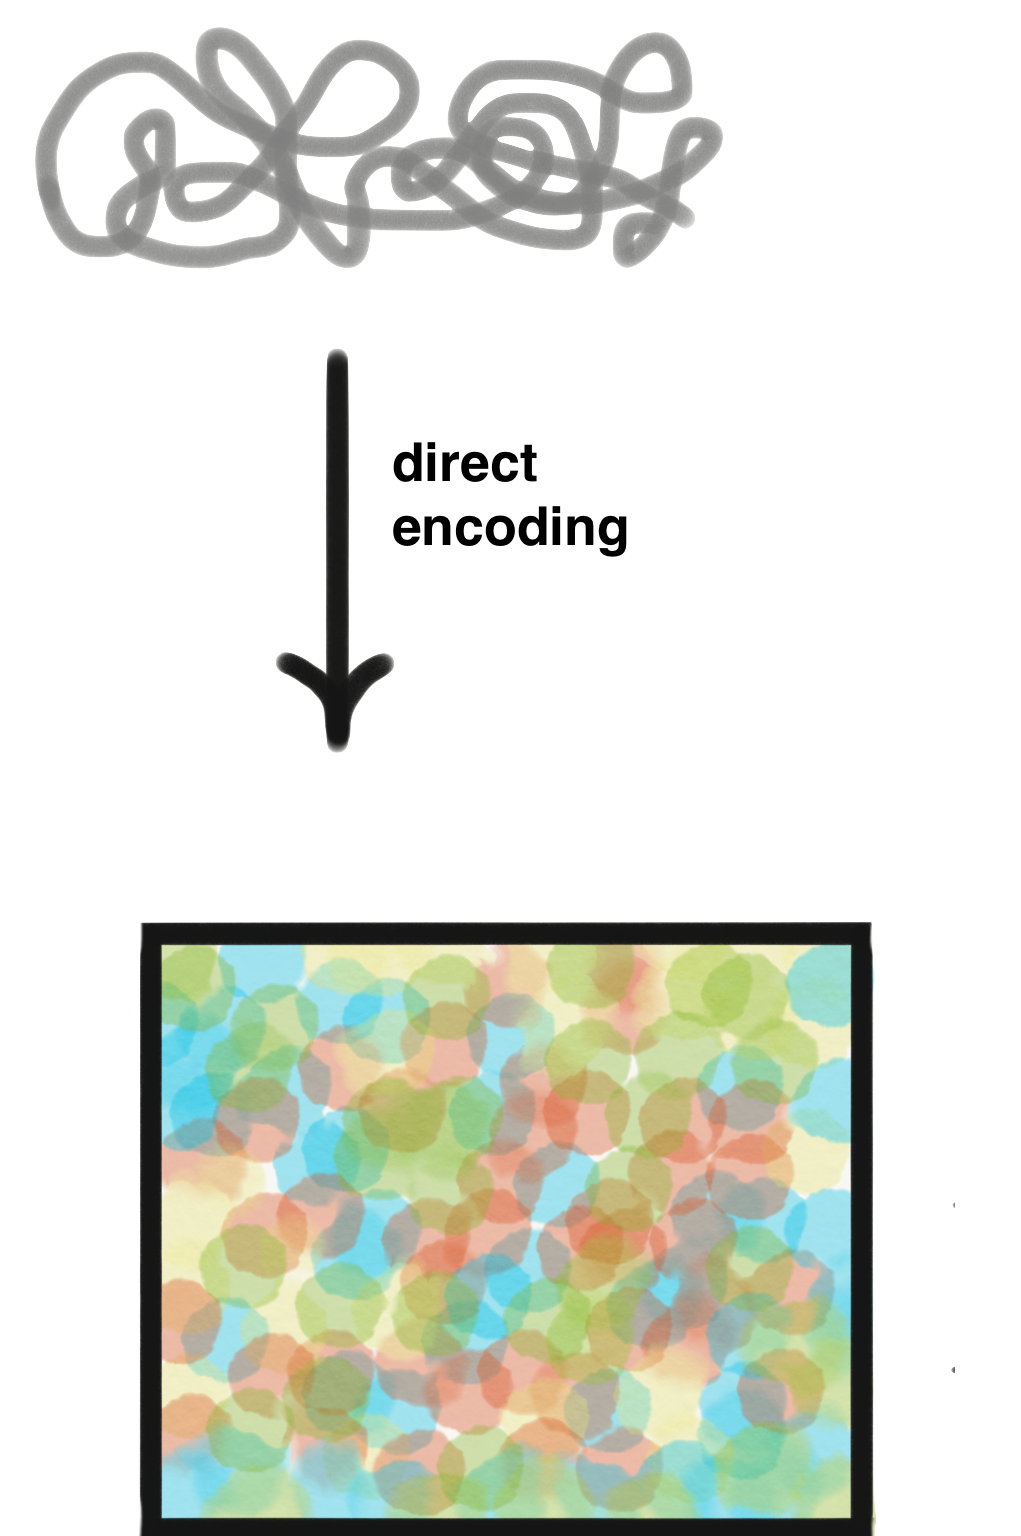
\includegraphics[width=\textwidth]{img/irregularity_direct_encoding.png}
        \caption{direct encoding}
        \label{subfig:direct_encoding}
    \end{subfigure}
    \hfill
    \begin{subfigure}[b]{0.4\textwidth}
        \centering
        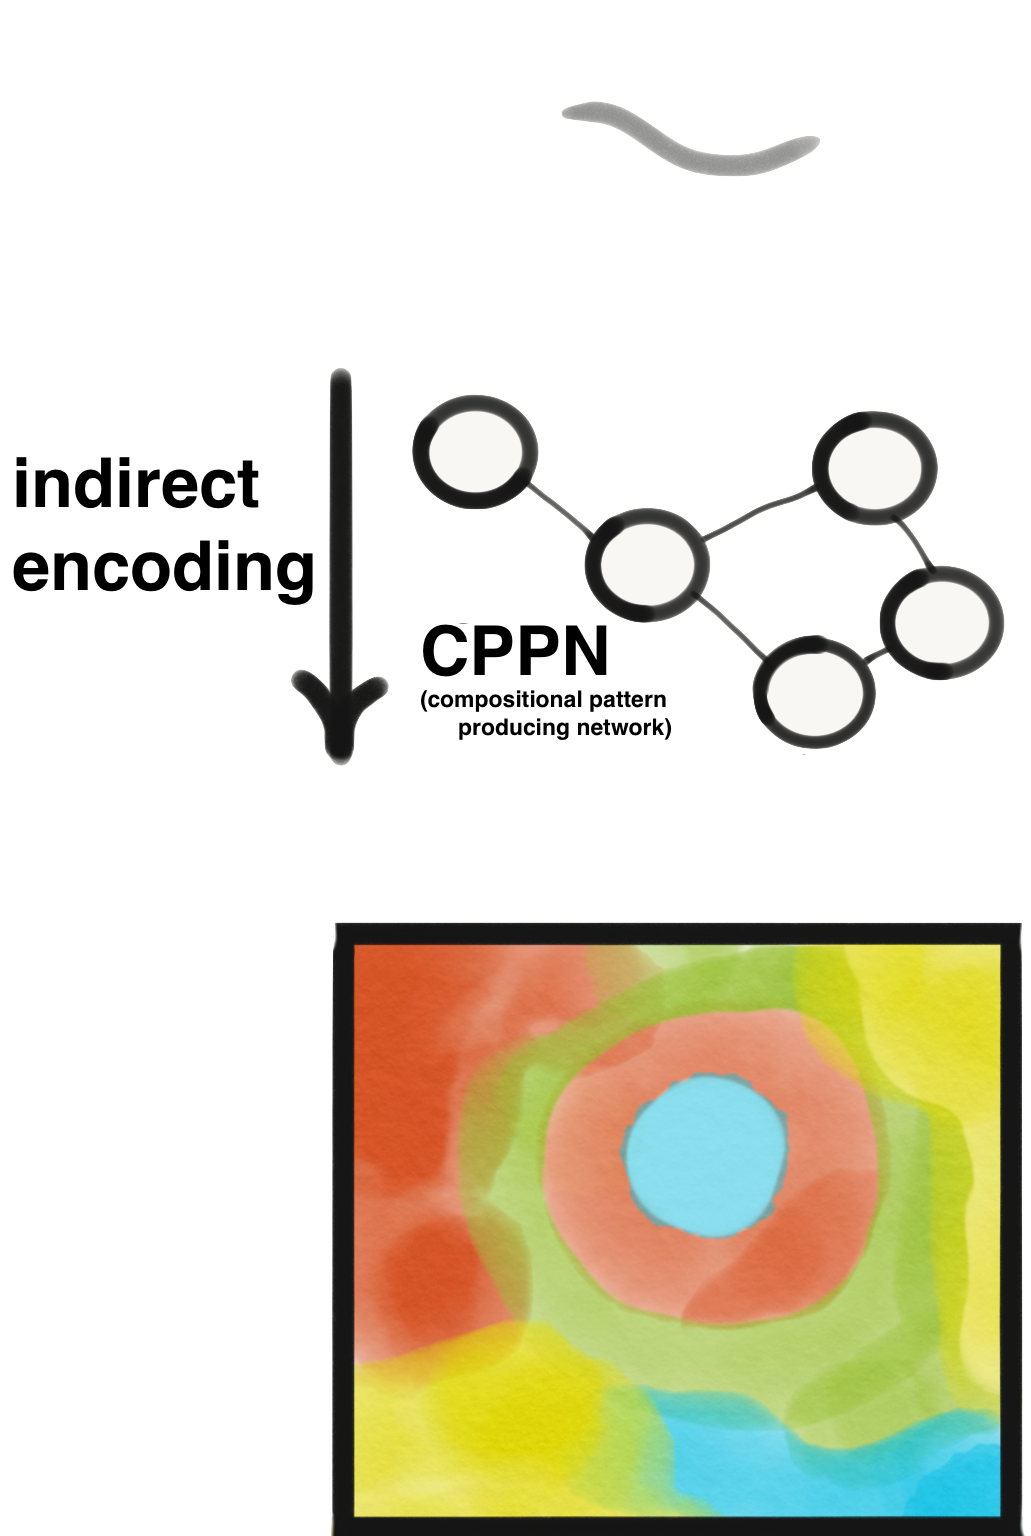
\includegraphics[width=\textwidth]{img/regular_indirect_encoding.png}
        \caption{indirect encoding}
        \label{subfig:indirect_encoding}
    \end{subfigure}
    \hfill
  \captionsetup{singlelinecheck=off,justification=raggedright}
  \caption[]{Archetypal examples of genotype to phenotype mapping from direct genetic representations and indirect phenotypic representations are illustrated. In both depictions, genetic information is shown at the top of the image and the corresponding phenotype is shown on the bottom of the image. In subfigure \ref{subfig:direct_encoding}, which depicts a direct encoding, a large volume of genetic information (where each characteristic of the phenotype is explicitly and independently described) is directly translated into a phenotype. Subfigure \ref{subfig:indirect_encoding} depicts an indirect encoding. In this particular scheme, a small amount of genetic information describes the configuration of a compositional pattern producing network (CPPN). This CPPN is then used to generate a phenotype.}
  \label{fig:indirect_bias}
\end{figure}